%---------------------------------------------------------%
%______//------             GAC             ------\\______%
%______||------         Chapitre 8          ------||______%
%______\\------   Propriétés géométriques   ------//______%
%---------------------------------------------------------%

\chapter{Propriétés géométriques}
\label{cha:propr-geom}

  Une propriété géométrique est une propriété invariante par quasi-isométries.


  \begin{defi}\index{Groupes!commensurables} 
    Deux groupes sont \emph{commensurables} s'ils possèdent des sous-groupes d'indice fini isomorphes.
  \end{defi}

  \begin{rems}
    \begin{enumerate}
    \item Pour les groupes finiment engendrés, deux groupes commensurables sont quasi-isométriques (à cause du
      corollaire précédent).
    \item En revanche, deux groupes quasi-isométriques n'implique pas qu'ils sont commensurables (en général).
    \end{enumerate}
  \end{rems}

  \begin{exs}
    \begin{enumerate}
    \item Si $F$ est un groupe fini, alors $\Z \times F$ et $D_\infty$ sont commensurables, car ils possèdent
      tous les deux le sous-groupe $\Z$ qui est d'indice fini.

    \item Pour $k, l \geq 2$, $\F_k$ est commensurable à $\F_l$.
    \end{enumerate}
  \end{exs}

  \begin{defi}
    Soit $(P)$ une propriété des groupes finiment engendrés. On dit que $G$ est \emph{virtuellement $(P)$}
    \index{Groupe!virtuellement $(P)$} si $G$ possède un sous-groupe $H$ d'indice fini qui a la propriété $(P)$.
  \end{defi}

  \begin{ex}[virtuellement libre]
    Si $G$ est virtuellement libre, alors $G$ possède un sous-groupe $H$ d'indice fini qui est libre.
  \end{ex}

  \begin{exs}
    \begin{enumerate}
    \item \og Être fini \og est une propriété géométrique. Car $G$ est fini ss'il est qi à $\{1\}$ et par
      transitivité, si $H$ est qi à $G$, il est aussi qi à $\{1\}$ et donc fini.

    \item \og Être cyclique infini\fg{}, c'est-à-dire \og être $\Z$\fg{}, n'est pas une propriété
      géométrique. $\Z$ et $\Z \times \Z/2\Z$ sont qi, mais le second n'est pas cyclique infini. De même pour
      $\Z$ et $D_\infty$.
    \end{enumerate}
  \end{exs}


  \begin{prop}
    \begin{enumerate}
    \item Être virtuellement $\Z$ est une propriété géométrique.
    \item Être virtuellement libre est une propriété géométrique.
    \item Être virtuellement abélien est une propriété géométrique.
    \item Avoir une présentation finie est une propriété géométrique.
    \item Avoir un problème des mots résolubles est une propriété géométrique.
    \item Être virtuellement nilpotent est une propriété géométrique.
    \end{enumerate}
  \end{prop}

  La proposition est difficile à prouver, mais pour quelques assertions, on peut le montrer en utilisant la
  croissance des groupes.

  \section{Croissance des groupes}
  \label{sec:croiss-des-groupes}
  
    Soit $G$ un groupe finiment engendré et $S = S^{-1}$ une partie finie symétrique génératrice de $G$.

    \begin{defi}
      La \emph{fonction de croissance} \index{Fonction!de croissance} de $G$ par rapport à $S$ est
        \[V_S: \N \to \R^+\ (\N^+),\ n \mapsto |B_S(n)| \]
      où $B_S(n) = \{g \in G\ |\ |g|_S \leq n\}$.
    \end{defi}

    \begin{exs}
      \begin{enumerate}
      \item Si $G$ est fini, alors $V_S(n)$ est constant pour $n \gg 0$

      \item Si $G = \Z$ et $S = \{\pm 1\}$,
        \begin{center}
          \begin{tikzpicture}
            \foreach \n in {-2, -1, ..., 2} {
              \draw (\n, 0.1) node[above]{$\n$} -- (\n, -0.1);
              \draw (\n, 0) -- ($(\n, 0) + (1, 0)$);
            }
            \draw (0,0) circle(1);
            \draw (3, 0) node[right]{$\Z$};
          \end{tikzpicture}
        \end{center}
        alors $V_s(n) = 2n + 1$.

      \item Si $G = \Z^2$ avec $S = \{(\pm 1, 0), (0, \pm 1)\}$,
        \begin{center}
          \begin{tikzpicture}
            \draw[->, >=latex] (-3, 0) -- (3, 0);
            \draw[->, >=latex] (0, -3) -- (0, 3);
            \draw (1, 0.1) node[above right]{$1$} -- (1, -0.1) (-0.1, 1) node[above right]{$1$} -- (0.1, 1);
            \draw[color=OliveGreen] circle(1);
            \draw[color=RoyalBlue] ({2/sqrt(2)}, 0) -- (0, {2/sqrt(2)}) -- ({-2/sqrt(2)}, 0) -- (0,
            {-2/sqrt(2)}) -- cycle;
            \draw[color=Red] ({2/sqrt(2)}, {2/sqrt(2)}) -- ({-2/sqrt(2)}, {2/sqrt(2)}) -- ({-2/sqrt(2)},
            {-2/sqrt(2)}) -- ({2/sqrt(2)}, {-2/sqrt(2)}) -- cycle;
            \draw (0,0) -- ({cos(45)}, {sin(45)}) node[midway, above left]{$\frac{n}{\sqrt{d}}$};
          \end{tikzpicture}
        \end{center}
        alors $V_S(n) = 1 + 4 \sum_{j=1}^n(n+1-j) = 2n^2 + 2n + 1 \leq (2n+1)^2$ (à vérifier).

      \item Si $G = \Z^d$ avec $S = \{(\pm 1, 0, \ldots, 0), \ldots, (0, 0, \ldots, \pm 1)\}$. Alors
        \[|B_S(n)| \leq (2n+1)^d,\ |B_S(n)| \geq \text{volume de la boule euclidienne de rayon }
        \frac{n}{\sqrt{d}} \cong C_dn^d.\]

      \item Si $G = \F_k$, $S = \{a_1^{\pm 1}, \ldots, a_k^{\pm 1}\}$. Soit $S(n) = \{g \in \F_k\ |\ |g|_S =
        n\}$. Alors $|S(n)| = 2k(2k-1)^{n-1}$ (car on a $2k$ choix pour la première lettre du mot, et ensuite
        comme on ne considère que des mots réduits, on a $2k-1$ choix pour le reste des lettres du mot). Ainsi
          \[V_S(n) = \sum_{i=0}^n |S(i)| = \cdots = \frac{k(2k-1)^n-1}{k-1}.\]
       \item Le groupe de Heisenberg discret.\index{Groupe!de Heisenberg discret}
         Si $A$ est un anneau commutatif à unité, le groupe de Heisenberg sur $A$ est 
         \[Heis(A) = \left\{
           \begin{pmatrix}
             1 & x & z \\ 0 & 1 & y \\ 0 & 0 & 1
           \end{pmatrix}\ |\ x,y,z \in A \right\} \subseteq GL_3(A).
         \]
         Considérons $Heis(\Z) = \langle a,b,c \rangle$.
           \[a =
           \begin{pmatrix}
             1 & 1 & 0 \\ 0 & 1 & 0 \\ 0 & 0 & 1
           \end{pmatrix},\ 
           b =
           \begin{pmatrix}
             1 & 0 & 0 \\ 0 & 1 & 1 \\ 0 & 0 & 1
           \end{pmatrix},\ 
           c =
           \begin{pmatrix}
             1 & 0 & 1 \\ 0 & 1 & 0 \\ 0 & 0 & 1
           \end{pmatrix}.
           \]
         On a que $[a,b] = c$, $[a,c] = [b, c] = 1$ (commutateurs). Ceci nous dit que $c$ commute avec $a$ et $b$.
         
         \textbf{Exercice:} Pour tous $m, n \in \Z$, $a^mb^n = c^{mn}b^na^n$ $(\ast)$ . Indication: démontrer que $a^m b
         = c^m ba^m$.
      \end{enumerate}
    \end{exs}

    \begin{rem}
      $(\ast)$ nous donne que tout $g \in G$ a une expression $g = a^mb^nc^p$ pour $m, n, p \in \Z$.
    \end{rem}

    \begin{prop}[Croissance du groupe de Heisenberg]
      Pour le groupe de Heisenberg, il existe des polynômes $P_1, P_2$ de degré 4 tels que
        \[\forall n \in \N, P_1(n) \leq V_S(n) \leq P_2(n).\]
    \end{prop}

    \begin{preuve}
      \begin{enumerate}
      \item Montrons que si si $g = a^m b^n c^p$, et $|g|_S \leq N$, alors $|m|, |n| \leq N$, $|p| \leq
        N^2$. En effet on au plus $(2N+1)$ choix pour $|m|$ et $|n|$ et $2N^2 + 1$ choix pour $|p|$, donc
          \[V_S(n) \leq (2N+1)^2(2N^2+1).\]
        L'application $\alpha : Heis(\Z) \to \Z^2$, $a^mb^nc^p \mapsto (m,n)$ est un homomorphisme de
        groupes. On a $a^mb^nc^pa^{m'}b^{n'}c^{p'} = a^{m+m'}b^{n+n'}c^\ast$. Ainsi $|\alpha(g)|_{\alpha(S)}
        \leq |g|_S \leq |g|_S$, c'est-à-dire $|m|+|n| \leq N$. 

        Montrons la seconde inégalité par récurrence sur $N$. Pour $N = 1$, c'est clairement bon. Soit $g' \in
        G$ avec $|g'|_S = N-1$, $g' = a^{m'}b^{n'}c^{p'}$. Alors on a un des trois cas:
        \begin{enumerate}
        \item $g = g' \cdot a^{\pm 1}$;
        \item $g = g' \cdot b^{\pm 1}$;
        \item $g = g' \cdot c^{\pm 1}$.
        \end{enumerate}
        \begin{enumerate}
        \item $g = g'a^{\pm 1} = a^{m'}b^{n'}c^{p'}a^{\pm 1} = a^{m'}b^{n'}a^{\pm 1}c^{p'} = a^{m'}c^{\pm
            n}a^{\pm 1} b^{n'} c^{p'} = \cdots = a^{m'\pm 1} b^{n'}c^{p'\pm n'}$.
            Comme $|p'| \leq (N-1)^2$, on a $|p'\pm n'| \leq (N-1)^2 + |n'| \leq (N-1)^2 + N \leq N^2$. 
            La deuxième inégalité est immédiate par récurrence.
        \item $g'b^{\pm 1} = a^{m'}b^{n' \pm 1} c^{p'}$. Comme $|p'| \leq (N-1)^2$, on a $|p'| \leq N^2$.
        \item $g'c^{\pm 1} = a^{m'}b^{n'}c^{p' \pm 1}$ et donc $|p' \pm 1 | \leq |p'| + 1 \leq (N-1)^2 + 1
          \leq N^2$. 
        \end{enumerate}
      \item Pour l'inégalité $P_1(n) \leq V_S(n)$, montrons que, si $m+n+6[\sqrt{p}] \leq N$ avec $m,n,p\geq
        0$, alors $|a^mb^nc^p|_S \leq N$. En effet, si $k^2 \leq p \leq (k+1)^2$, on a $a^mb^nc^p =
        a^mb^nc^{k^2}c^{p-k^2} = a^mb^n[a^k,b^k]c^{p-k^2}$, donc $|a^mb^nc^p| \leq m + n + 4k + p-k^2 < m + n
        + 4k + 2k + 1 \leq m +  n + 6k \leq N$.
        
        \textbf{Exercice:} $\iiint_{x+y+6\sqrt{z} \leq N,\ x,y,z \geq 0} 1dxdydz = kN^4$ avec $k$ constante.
      \end{enumerate}
    \end{preuve}


    \begin{defi}
      Soient $f, g: \R^+ \to \R^+$. Alors $f \prec g$ s'il existe $a, b, c \in \R$, $c, a > 0$ avec $f(x) \leq
      cg(ax+b)$ pour $x \gg 0$.
      On dit que $f \approx g$ si $f \prec g$ et $g \prec f$.
    \end{defi}

    \begin{exercice}
      Si $f, g$ sont des polynômes de même degré, alors $f \approx g$.
    \end{exercice}

    \begin{prop}[Équivalence de croissance]
      Soient $(G_1, S)$ et $(G_2, T)$ deux groupes quasi-isométriques (par exemples $S, T$ deux parties
      génératrices finies du même groupe $G$). Alors $V_S \approx V_T$.
    \end{prop}

    \begin{preuve}
      Soit $f: G_1 \to G_2$ une quasi-isométrie, c'est-à-dire qu'il existe $\lambda > 0$, $c \geq 0$ telles
      que pour tous $x, y \in G_1$
        \[\frac{1}{\lambda} |x^{-1}y|_S - c \leq |f(x)^{-1}f(y)|_T \leq \lambda |x^{-1}y|_S + c.\]

        \begin{center}
          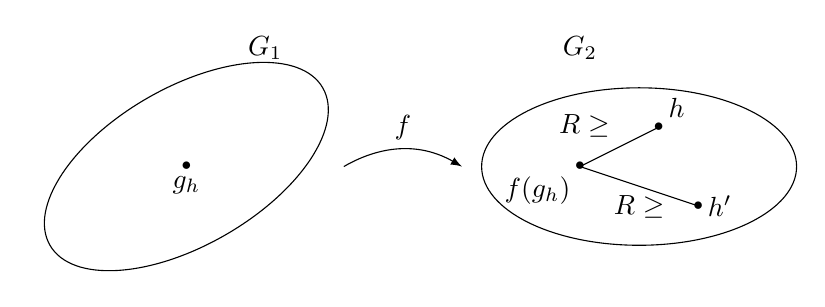
\begin{tikzpicture}
            \draw (0,0) node[scale=0.7]{$\bullet$} node[below]{$g_h$};
            \draw (6,0.5) node[scale=0.7]{$\bullet$} node[above right]{$h$};
            \draw (5, 0) node[scale=0.7]{$\bullet$} node[below left]{$f(g_h)$};
            \draw (6.5, -0.5) node[scale=0.7]{$\bullet$} node[right]{$h'$};
            \draw[rotate=30] (0, 0) ellipse(2cm and 1cm);
            \draw (5.75, 0) ellipse(2cm and 1cm);
            \draw (6, 0.5) to node[midway, above left]{$R \geq$} (5, 0);
            \draw (5, 0) to node[midway, below]{$R \geq$} (6.5, -0.5);
            \draw[->, >=latex] (2, 0) to[bend left] node[midway, above]{$f$} (3.5, 0);
            \draw (1, 1.5) node{$G_1$};
            \draw (5, 1.5) node{$G_2$};
          \end{tikzpicture}
        \end{center}
      On peut supposer $f(1_{G_1}) = 1_{G_2}$ (remplacer $f$ par $(f(1))^{-1}f)$. Donc $\frac{1}{\lambda}|y|_S
      - c \leq |f(y)|_T \leq \lambda |y|_S + c$ pour tout $y \in G_1$. Soit $R \geq 0$ tel que pour tout $h \in
      G_2$, il existe $g \in G_1$ tel que $|f(g)^{-1}h|_T \leq R$ (quasi-surjectivité).
      
      Pour chaque $h$ dans $G_2$, on choisit $g_h \in G_1$ tel que $f(g_h)^{-1}h|_T \leq R$. Pour $h \in
      B_T(n)$, on a $|g_h|_S \leq \lambda (|f(g_h)|_T + c)\ ( \iff \frac{1}{\lambda}|g_h|-c \leq |f(g_h)|) \leq
      \lambda (R+n+c)$ par l'inégalité du triangle. Pour $h$ fixé, le nombre de $h'$ avec $g_h = g_{h'}$ est
      au plus $|B_T(h, 2R) = V_T(2R)$.

      Donc $V_T(n) \leq \left| \{g_h\ |\ h \in B_T(n)\} \right| V_T(2R) \leq V_S(\lambda R + \lambda n +
      \lambda c)V_T(2R)$, qui est exactement la définition de $V_T \prec V_S$.
      
      Par symétrie on a $V_S \prec V_T$, d'où $V_S \approx V_T$.
    \end{preuve}


    \begin{defi}
      \begin{enumerate}
      \item La \emph{suite dérivée} \index{Suite!dérivée} de $G$ est définie par 
        \[G = G^{(0)} \supset G^{(1)} = [G,G] \supset \cdots \supset G^{(k)} = [G^{(k-1)}, G^{(k-1)}] \supset \cdots.\]
      \item La \emph{suite descendante} \index{Suite!descendante} de $G$ est 
          \[G = G_0 \supset G_1 = [G_0, G_0] \supset [G, G_1] \supset \cdots \supset G_k = [G, G_{k-1}]
          \supset \cdots.\]
      \end{enumerate}
      On a donc que $G^{(k)} < G_k$.
    \end{defi}

    \begin{defi}
      \begin{enumerate}
      \item On dit que $G$ est \emph{résoluble} \index{Groupe!résoluble} s'il existe $k \geq 1$ tel que
        $G^{(k)} = \{1\}$.

      \item On dit que $G$ est \emph{nilpotent} \index{Groupe!nilpotent} s'il existe $k \geq 1$ tel que $G_k = \{1\}$.
      \end{enumerate}
    \end{defi}


    On observe ainsi que si $G$ est nilpotent, alors $G$ est résoluble.

    \begin{exs}
      \begin{enumerate}
      \item Tout groupe abélien est nilpotent (donc résoluble).

        \begin{center}
          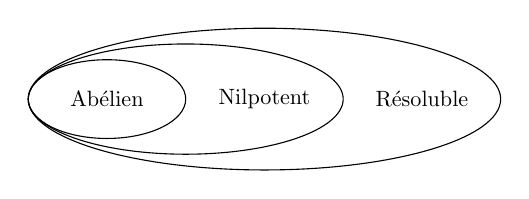
\begin{tikzpicture}
            \draw (0,0) ellipse (1cm and 0.5cm);
            \draw (0,0) node[scale=0.8]{Abélien};
            \draw (1,0) ellipse (2cm and 0.7cm);
            \draw (2,0) node[scale=0.8]{Nilpotent};
            \draw (2,0) ellipse (3cm and 0.9cm);
            \draw (4,0) node[scale=0.8]{Résoluble};
          \end{tikzpicture}
        \end{center}

      \item Pour tout anneau commutatif à unité $A$, le groupe de Heisenberg $Heis(A)$ est nilpotent, car 
          \[[Heis(A), Heis(a)] \subset \left\{
            \begin{pmatrix}
              1 & 0 & z\\ 0 & 1 & 0\\ 0 & 0 & 1
            \end{pmatrix}\ \big|\ z\in A \right\} = Z(Heis(A))
          \]
        le centre de $Heis(A)$ (pour rappel, $Z(G) = \{g \in G\ |\ [g,h] = 1\ \forall h \in G\}$. De plus
          \[Heis(A) \supset [Heis(A), Heis(A)] \supset [Heis(A), \underbrace{[Heis(A), Heis(A)]}_{\subset
            Z(Heis(A))}] = \{1\}\]
        car le centre commute avec tous les éléments.
      \end{enumerate}
    \end{exs}

    \begin{prop}
      Soit $G$ un groupe nilpotent.
      \begin{enumerate}
      \item $G_{j+1} \lhd G_j$
      \item $G_j/G_{j+1}$ est abélien.
      \end{enumerate}
    \end{prop}
    

    \begin{preuve}
      Exercice.
    \end{preuve}

    
    En 1972, Hyman \textsc{Bass} démontre que tout groupe virtuellement nilpotent de présentation finie est à
    croissance polynomiale (avec un calcul explicite du degré de croissance).

    \begin{defi} \index{Rang} 
      Pour $A$ abélien et finiment engendré, $A = \Z \oplus F$ où $|F| < \infty$ (voir
      la structure du groupe abélien), on définit le \emph{rang} comme 
        \[\rk_{\Z} A = r.\]
    \end{defi}


    \begin{theo}[de \textsc{Bass}] \index{Théorème!de Bass} \index{Degré de nilpotence}
      Soit $G$ un groupe nilpotent finiment engendré. Soit $n \in \N$ le minimum tel que $G_N = \{1\}$ (ce $n$
      s'appelle \emph{degré de nilpotence}). La fonction de croissance de $G$ est polynomiale de degré
        \[\sum_{j=0}^{n-1}(j+1)\rk_{\Z}\left(G_j/G_{j+1}\right).\]
    \end{theo}

    \begin{cor}
      Soit $G$ virtuellement nilpotent. Alors $G$ a une croissance polynomiale.
    \end{cor}

    \begin{theo}[de \textsc{Gromov}] \index{Théorème!de Gromov}
      Soit $G$ un groupe finiment engendré à croissance polynomiale. Alors $G$ est virtuellement nilpotent.
    \end{theo}

    Le preuve de ce théorème a fondé la plupart des techniques actuelles de géométrie des groupes.

    \begin{cor}
      ``Être virtuellement nilpotent'' est une propriété géométrique. {\normalfont \small[pour rappel, une propriété
        géométrique est une propriété invariante par qi. Si $A$ qi à $B$ et si $A$ a une propriété
        géométrique, alors $B$ l'a aussi.]}
    \end{cor}

    \begin{preuve}
      Soit $G_1$ quasi-isométrique à $G_2$ et soit $G_1$ virtuellement nilpotent. Par le corollaire ci-dessus,
      $G_1$ a une croissance polynomiale. Par la proposition d'équivalence des croissances, $G_2$ a une
      croissance polynomiale aussi. Ainsi par Gromov, $G_2$ est virtuellement nilpotent.
    \end{preuve}


    \begin{cor}
      ``Être virtuellement $\Z$ (cyclique)'' est une propriété géométrique.
    \end{cor}


    \begin{preuve}
      Soit $G$ quasi-isométrique à $\Z$. Alors $G$ a une croissance linéaire. En effet, dans $\Z$, les boules
      $V(n) = 2n + 1$, qui est linaire. Comme une croissance linéaire est une croissance polynomiale, $G$ est
      virtuellement nilpotent par Gromov.

      Soit alors $H \leq G$ un sous-groupe d'indice fini tel que $H$ est nilpotent. $H$ a aussi une croissance
      linéaire car la croissance d'un sous-groupe ne peut pas être plus grande que celle du groupe. Par Bass,
      on a
        \[1 = \sum_{j=0}^{n-1}(j+1)\rk_{\Z}\left(H_j/H_{j+1}\right)\]
      où $n$ est le degré de nilpotence.

      Comme $j+1$ et le rang sont tous deux positifs, la seule possibilité est que $\rk_{\Z}\left(H_0/H_1\right)
      = 1$ et $\rk_{\Z}\left(H_j/H_{j+1}\right) = 0$ pour tout $j \geq 1$, on a $H_0 = H$. Ainsi
      \[H_0/H_1 = H/[H, H] \cong \Z \oplus F,\ |F| < \infty.\]
      $H_1/H_2 = [H, H]/[H, [H, H]]$ est fini, on regarde tous les quotients et on arrive à un moment à
      $H_n = \{1\}$, ainsi $H_{n-1} / H_n = H_{n-1}/\{1\}$ est fini, donc $H_{n-1}$ est fini. Ceci montre que
      $H_i$ est fini pour chaque $i$, donc c'est vrai en particulier pour $H_1$. Donc
      $H_0/H_1 = H/\mathrm{fini} \cong \Z \oplus F$ qui montre que $H$ est virtuellement $\Z$, et donc $G$ est
      aussi virtuellement $\Z$ par Milnor-\v{S}varc.
    \end{preuve}



    En 1983, R. \textsc{Grigorchuck} a constuit le premier exemple d'un groupe $(G, S)$ à \emph{croissance
      intermédiaire}, et a montré que
      \[e^{\sqrt{n}} < V_S(n) < e^{n^{0.991}}.\]

    On a vu (Gromov et Bass) que la croissance polynomiale est équivalente pour un groupe à être virtuellement
    nilpotent. La croissance polynomiale est plus petite que la croissance intermédiaire (Grigorchuck),
    elle-même plus petite que la croissance exponentielle (presque tous les groupes ont une croissance
    exponentielle).




    \begin{defi} \index{Série!de croissance}
      Soit $G$ un groupe finiment avec une partie génératrice finie $S$. La \emph{série de croissance} de $G$
      par rapport à $S$ est
        \[f_{(G,S)}(z) = \sum_{n \geq 0}a_nz^n\]
      où $a_n = \left| \{g \in G\ |\ |g|_S = n\} \right|$ (mots de longueur $n$). On peut aussi parler de $b_n
      = V_S(n) = \left| \{g \in G\ |\ |g|_S \leq n\} \right|$ à la place de $a_n$.
    \end{defi}

    
    \textbf{Question:} existe-t-il des groupes avec une croissance rationelle, i.e. est-ce que $f(z)$ peut
    s'exprimer comme quotient de polynômes $P(z), Q(z) \in \Z[z]$?


    \begin{theo}
      Soit $G$ un groupe, $G = \langle S \rangle$ avec $|S| < \infty$. Si $G$ a un language de formes normales
      qui est régulier, alors la série $f_{(G, S)}(z)$ est rationnelle.
    \end{theo}

    \begin{defi}
      On appelle \emph{formes normales} \index{Forme normale} le fait de prendre un mot sur $S$ pour chaque
      élément dans $G$.
    \end{defi}

    \begin{exs}
      \begin{enumerate}
      \item Considérons $\Z^2$ avec le système de générateurs $\{a^{\pm 1}, b^{\pm 1}\}$. Un langage de
        formes normales est $\{a^nb^m,\ n, m \in \Z\}$.

      \item Considérons le groupe libre $(\F_2, \{a^{\pm 1}, b^{\pm 1}\})$. Un langage de formes normales est
        donné par tous les mots réduits (c'est le langage naturel sur le groupe libre).
      \end{enumerate}
    \end{exs}


    
    

    

    
    



    

    

    


%%% Local Variables:
%%% mode: latex
%%% TeX-master: "../GAC_cours.tex" 
%%% End: